 \thispagestyle{empty}
 \lhead{Research Proposal: Post Quantum Hardware Cryptography and Homomorphic  Encryption}
 \phantom \quad \\
\hrule \phantom \quad  \vspace*{1\baselineskip}  \\
 {\bf Research Proposal: Post Quantum Hardware Cryptography and Homomorphic  Encryption}
 \vspace*{1\baselineskip}  \hrule \phantom \quad \\


\begin {itemize}
 \item [$\bullet$] { \bf Summary:} \vspace{0.5em} \\
This research program focuses on simplifying the complexity and ensuring efficient hardware implementation of post-quantum cryptography, homomorphic encryption, and homomorphic data processing embedded systems.

 \item [$\bullet$] { \bf Introduction:} \vspace{0.5em} \\
This research proposal aims to address two aspects of concern related to modern communication devices and systems. The first aspect is security, and the second aspect is privacy.
\begin{itemize}
\item [-]
Security: \\ Cryptographic systems have become integral components of nearly every communication device, providing confidentiality, data security, and authentication in various applications such as communication devices, autonomous vehicles, the Internet of Things (IoT), and healthcare [1,2,3,4]. However, the advent of quantum computers capable of executing the Shor algorithm [5] poses a threat to popular public key cryptography systems like RSA and elliptic curve cryptography. This jeopardizes the security of digital communications and exposes user data. The National Institute of Standards and Technology (NIST) has initiated a competition for developing cryptographic systems resistant to quantum computer attacks, with round 3 submissions currently underway [6].
\item [-]
Privacy: \\ Another issue arising from the expansion of the Internet and cloud systems is privacy concern. Despite secure communication between user computers and cloud systems, data is still decrypted in the cloud for processing. Consequently, third parties with access can read and exploit the data. Homomorphic Encryption (HE), introduced by Gentry, is a privacy-preserving algorithm enabling computation over encrypted data without decryption.
\end{itemize}
As these algorithms are expected to shape future cryptographic systems, designing efficient embedded systems for their implementation is crucial. In the next section, I elaborate on my methods to address this challenge.
 \item [$\bullet$] { \bf Challenges:} \vspace{0.5em} \\
 In this section, the challenges ahead of  Post-Quantum Cryptography (PQC) and Homomorphic Encryption (HE) is briefly explained and how this research proposal tries to address these challenges.
 
 
 
 Post-quantum cryptography  are believed to be secure against attacks by quantum computers.  While post-quantum cryptography aims to provide alternatives that resist quantum attacks, it also faces several challenges:
\begin{itemize}

 \item[-]   Standardization: There is not yet a widely accepted standard for post-quantum cryptographic algorithms. 
 \item[-]  Migration: Transitioning from existing cryptographic systems to post-quantum cryptography poses challenges. It requires updating protocols, systems, and infrastructure across various applications and services, which can be a time-consuming and complex process.
 \item[-]     Performance: Many post-quantum cryptographic algorithms are computationally more intensive than current algorithms, potentially leading to performance challenges, especially in resource-constrained environments. Researchers are working to optimize these algorithms to improve efficiency.
  \item[-]    Implementation Issues: Implementing cryptographic algorithms correctly is crucial for security. However, there's a risk that poorly implemented post-quantum algorithms may introduce vulnerabilities. Ensuring secure and correct implementations is a challenge, especially given the complexity of some post-quantum cryptographic schemes.
  \item[-]    Lack of Real-World Testing: Post-quantum cryptographic algorithms are relatively new, and their real-world performance and security need to be validated through extensive testing and deployment. Until these algorithms are widely deployed and tested, their effectiveness and resilience against both quantum and classical attacks remain theoretical.
  \item[-]    Quantum-Safe Key Management: Post-quantum cryptographic systems rely on key exchange mechanisms, and secure key management is crucial. Quantum-safe key exchange protocols need to be developed and integrated into existing systems to ensure that keys remain secure even in a post-quantum world.
 \item[-]     Evolving Threat Landscape: The threat landscape is dynamic, and adversaries may adapt their strategies and techniques. Post-quantum cryptographic algorithms need to be resilient not only to known quantum attacks but also to potential new attack vectors that may emerge.
  \item[-]    Global Adoption: Achieving global adoption of post-quantum cryptographic standards is a challenge. Different countries and organizations may have varying levels of readiness and priorities, and achieving a coordinated transition is essential for overall security.
 \end{itemize}
 
 
 
 
Homomorphic encryption  provides a significant advantage for privacy and security in scenarios where sensitive data needs to be processed in a secure manner. However, homomorphic decryption, or more accurately, the challenge associated with homomorphic encryption, involves several factors:
\begin{itemize}

  \item[-]   Computational Overhead: Homomorphic encryption typically introduces a significant computational overhead. Performing operations on encrypted data is computationally more intensive than on the equivalent unencrypted data. This can lead to slower processing times, making it less practical for certain applications.

 \item[-]    Key Management: Managing the keys used in homomorphic encryption is crucial. If keys are compromised, it can potentially lead to the compromise of the entire encrypted data. Key management becomes even more challenging as the complexity of the homomorphic encryption scheme increases.

 \item[-]    Limited Functionality: While homomorphic encryption allows for certain types of computations on encrypted data, it may not support all types of operations. Some computations, particularly those involving complex data structures or iterative algorithms, can be challenging to perform efficiently in a homomorphically encrypted domain.

  \item[-]   Size Expansion: Homomorphic encryption can cause significant expansion in the size of the encrypted data compared to the original unencrypted data. This can be a concern, especially when dealing with large datasets.

   \item[-]  Adaptation of Applications: Existing applications and algorithms may need to be adapted or restructured to work with homomorphic encryption. This can be a barrier to the widespread adoption of this technology.
\end{itemize}

 \item [$\bullet$] { \bf Proposed Research:} \vspace{0.5em} \\
This research objective is to develop a novel hardware-based solution aimed at addressing  challenge such as Performance, Implementation Issues, Lack of Real-World Testing, Quantum-Safe Key management. The key characteristics of the proposed encryption hardware is listed below:
\begin{itemize}
   \item[-]   Design and implement a hardware accelerator for post-quantum cryptographic algorithms to enhance performance.
   \item[-]   Address implementation challenges, ensuring robustness against side-channel attacks, fault-injection attacks, Differential Power Analysis (DPA), and Tempest Attacks.
  \item[-]    Conduct extensive real-world testing to validate the effectiveness and practicality of the proposed hardware solution.
  \item[-]    Develop quantum-safe key management protocols suitable for integration into existing cryptographic systems.
\end {itemize}
Regarding the HE, the main objective of this research would be to design a hardware capable of the performing neural network inference on the encrypted data. The hardware focus would be on efficient addition and subtraction. Leverage parallel processing capabilities and optimized memory management to enhance overall performance.The objectives of this research are:
    \begin{itemize}
    \item[-]    Break down neural network inference computations into homomorphic encryption-supported operations, emphasizing addition, subtraction, and minimizing multiplications.
  \item[-]   Design a specialized hardware accelerator targeting homomorphic encryption operations to significantly improve computational efficiency.
  \item[-]   Mitigate key management challenges associated with homomorphic encryption, ensuring secure and efficient use.
  \item[-]   Adapt the proposed hardware accelerator for seamless integration into neural network applications
    \end{itemize}
 \item [$\bullet$] { \bf Method:} \vspace{0.5em} \\
  The methodology to carry out  the PQC research proposal could be breakdown into following phases:
 \begin{itemize}
 \item [-]  Phase 1, Hardware Design and Verification: Design a specialized hardware architecture optimized for PQC encryption, focusing on enhancing performance while minimizing costs. Considerations will include parallel processing capabilities, efficient memory management, and power consumption optimization.
 \item [-]  Phase 2, Implementation Robustness: Implement countermeasures against common cryptographic attacks, including side-channel attacks, fault-injection attacks, DPA, and Tempest Attacks. Employ techniques such as secure coding practices, constant-time algorithms, and hardware-based protections to fortify the implementation against potential vulnerabilities.
  \item [-]  Phase 3, Real-World Testing:
Conduct comprehensive real-world testing in various scenarios to evaluate the proposed hardware's performance, scalability, and compatibility with existing systems. Collaborate with industry partners and organizations to simulate diverse deployment environments.
  \item [-]  Phase 4, Quantum-Safe Key Management:
Develop and implement quantum-safe key management protocols that ensure the security and integrity of cryptographic keys. Evaluate the resilience of these protocols against both classical and quantum attacks.
 \end{itemize}
 The methodology to carry out the HE research proposal could be breakdown into phases:
     \begin{itemize}
     \item [-]  Phase 1, Neural Network Optimization: Explore the methods (such as sparsity) to minimize the number of computations required to perform inference. Since, the HE computations are expensive, this phase can significantly improve the overall performance. 
     \item [-]  Phase 2, Operation Breakdown: Analyze neural network inference computations to identify opportunities for minimizing multiplicative operations. Propose strategies to restructure computations and replace multiplications with more homomorphic encryption-friendly additions and subtractions.
     \item [-] Phase 3, Implementation: This phase aims to implement the HE based neural network inference engine on hardware. In this research proposal, Field Programmable Gate Arrays (FPGAs) are chosen as the initial implementation target for their reconfigurability, affordability, and speed.
      
      \item [-] Phase 4, Verification and Testing: This phase aims to test the designed hardware and verify the functionality. The patterns are encrypted using He algorithms and would serve as inputs to test the HE based NN inference engine. The obtained accuracy should be closed to the accuracy obtained from the hardware. 
            \item [-] Phase 5, Real-world Application: Explore methods to seamlessly integrate the designed hardware accelerator into existing neural network applications. Address compatibility issues and provide adaptation guidelines to facilitate widespread adoption.
     \end{itemize}
%\item [-]
 \item [$\bullet$] { \bf Current Research:} \vspace{0.5em} \\
While working as a postdoctoral researcher at the University of Windsor, I began my research in cryptography by focusing on creating efficient hardware for multiplying binary polynomials. The results of this project were successfully published in a well-known journal.

Afterwards, I shifted my focus to Post-Quantum Cryptography (PQC) and Homomorphic Encryption (HE) algorithms. I worked on improving the efficiency of hardware for multiplying large integer polynomials, a crucial aspect in PQC and HE cryptography systems. Specifically, I addressed the challenge of slow and resource-intensive polynomial multiplication by using the Number Theoretic Transform (NTT), a widely adopted algorithm.

This work was completed during my part-time role as a researcher at the University of Windsor, resulting in the filing of a provisional patent. Currently, we are working on obtaining a patent for the developed circuit. Additionally, a circuit was developed based on this concept to perform hardware multiplication of extremely large integers for Fully Homomorphic Encryption (FHE), addressing the challenge of dealing with very large numbers. This research in under review for publication. 

Regarding the Neural Networks, where I strategically utilized sparsity to achieve a significant reduction in the number of parameters by almost 80$\%$, without compromising accuracy. This reduction substantially lowered the computation required for inference tasks. The overarching goal is to apply these techniques to reduce computational requirements when performing inference on the encrypted data using HE.
 \item [$\bullet$] { \bf Research Program Feasibility:} \vspace{0.5em} \\
 The first phase involves optimizing algorithms for hardware implementation using Python for simulations and FPGAs for efficiency measurement. FPGAs, being cost-effective and flexible, are advantageous over designing and fabricating a VLSI ASIC. After testing, the design can be fabricated for final evaluations. Three defined projects include studying post-quantum cryptographic algorithms, investigating homomorphic encryption and ciphertext computation algorithms, and designing an architecture and circuit for efficient hardware implementation.
 \item [$\bullet$] { \bf Funding and Grant Potential:} \vspace{0.5em} \\
Leveraging my industry background and familiarity with industry problems, I plan to secure funding for the research. I have successfully written research proposals with industry partners to obtain MITACS grants in the past. 
       
\begin{itemize}
\item [-]
    Natural Sciences and Engineering Research Council of Canada (NSERC):
        NSERC provides grants to support research in natural sciences and engineering, including computer science and cryptography.
%\item [-]
%    Canadian Cyber Threat Exchange (CCTX):
%        CCTX focuses on cybersecurity initiatives and may have funding opportunities for research related to cryptographic solutions and encryption technologies.

\item [-] Tech Companies:

    IBM Research: Companies like IBM have research divisions that may fund projects related to cryptography and encryption.\\
    Microsoft Research: Microsoft has an interest in various areas of cryptography and may provide research grants.
\item [-]
    Canadian Institutes of Health Research (CIHR):
        CIHR may provide funding for research projects that involve the intersection of health data and encryption technologies.
\item [-]
    Mitacs:
        Mitacs offers collaborative research internships and training programs that connect researchers with industry partners. It could be a valuable resource for projects with practical applications.
\item [-]
    Canada Foundation for Innovation (CFI):
        CFI supports state-of-the-art infrastructure for research. If your project involves the development of specialized equipment or facilities, CFI might be a relevant funding source.
%\item [-]
%    Canadian Security Establishment (CSE):
%        CSE is focused on cybersecurity and may have opportunities for collaborative research projects in the area of encryption and secure communication.
\item [-]
    Defence Research and Development Canada (DRDC):
        DRDC, as the research arm of the Canadian Department of National Defence, may fund projects related to cryptographic solutions with applications in defense and security.
%\item [-]
%    Information and Communications Technology Council (ICTC):
%        ICTC focuses on advancing Canada's digital economy and workforce. They may support research projects that contribute to the advancement of encryption technologies.
\item [-]
    Federal Economic Development Agency for Southern Ontario (FedDev):
        Ontario support academic research in emerging technologies through FedDev.
\end{itemize}

 \end {itemize}
\hspace*{-1.8em}
{\bf References} \\
%\vspace*{-4em}
{\footnotesize
\begin{itemize}
\item[] [1] J. Yoo and J. H. Yi, “Code-based authentication scheme for lightweight integrity checking of smart vehicles,” IEEE Access,
vol. 6, pp. 46731–46741, 2018.
\item[] [2] R. Abu-Salma, M. A. Sasse, J. Bonneau, A. Danilova, A. Naiakshina, and M. Smith, “Obstacles to the adoption of secure
communication tools,” in 2017 IEEE Symposium on Security and Privacy (SP), pp. 137–153, 2017.
\item[] [3] P. Aparna and P. V. V. Kishore, “Biometric-based efficient medical image watermarking in e-healthcare application,” IET
Image Processing, vol. 13, no. 3, pp. 421–428, 2019.
\item[] [4] T. D. P. Bai, K. M. Raj, and S. A. Rabara, “Elliptic curve cryptography based security framework for internet of things (iot)
enabled smart card,” in 2017 World Congress on Computing and Communication Technologies (WCCCT), pp. 43–46, 2017.
\item[] [5] P. W. Shor, "Algorithms for quantum computation: discrete logarithms and factoring," Proceedings 35th Annual Symposium on Foundations of Computer Science, 1994, pp. 124-134, doi: 10.1109/SFCS.1994.365700
\item[] [6] “Post-Quantum Cryptography-Round 3 Submissions,” 2024.
\end{itemize}


}


%\end{itemize}


%{\bf Case II: 
%Post Quantum Hardware Cryptography and Homomorphic  Encryption}\\
%%\vspace*{3\baselineskip}\\
%This research program involves reducing complexity and efficient hardware implementation of the post quantum cryptography, homomorphic encryption, and homomorphic data processing embedded systems. \\[0.2cm]
%{\bf Background:  } 
%Cryptography systems have become  inseparable parts of almost every communication device.
%Cryptography is  used to provide confidentiality, data security, and authentication in many applications such as
%communication devices, autonomous vehicles, Internet of Things (IoT), healthcare [1,2,3,4] etc.


%However, with rise of the quantum computers capable of executing Shor algorithm  [5], many popular public key cryptography systems including RSA  and elliptic curve cryptography will be no longer secure.  This would greatly endanger the security of digital communications and expose user's data. 
% National Institute of Standards and Technology (NIST) has already started a competition for developing cryptographic systems that are resistant to quantum computers attacks. At present, NIST has called for submissions for round 3 of this completion [6]. 
%%The submission for previous rounds could be find in references \citecrypto{nistr2,nistr1}. 


%Another issue with expansion of the Internet and cloud systems is privacy concern. 
% Currently, with the most secure communication between user computer and cloud system, still the data is decrypted in the cloud for processing. Therefore, the third parties owning the cloud and those with authorized access can read the data and use it for their own advantages. Homomorphic Encryption (HE), first introduced by Gentry  is a privacy preserving algorithm that allows valid computing over encrypted data without the need to decrypting it. 
% 
% Since these algorithms are expected to be the future  cryptography systems, it is important to design an efficient  embedded systems for these systems. In next section,
% I further explain my methods to address this challenge. \\
%{\bf Method: } 
%Since  post quantum cryptography is a rather new field and because of  complexity of its algorithms, there exists only a limited number of the hardware implementations for these algorithms. 
% In this research proposal, Field Programmable Gate Arrays is selected as the initial implementation target since they provide a  reconfigurable, cheap and yet fast hardware platform. 
% % Round 3  finalists for public-key encryption, key establishment and digital signature are already available in NIST website. Most of these algorithms come only with a software implementation. Even those with hardware implementation still have plenty of room for improvement. This also applies to homomorphic encryption and computation as I discuss it further in the following. 
%  In homomorphic encryption, plaintext is transformed into ciphertext, allowing computation on the encrypted data resulting in another ciphertext. Decryption of this ciphertext yields the same computation result as if it had been performed on plaintext.
% % \begin{figure}
%% \centering
%%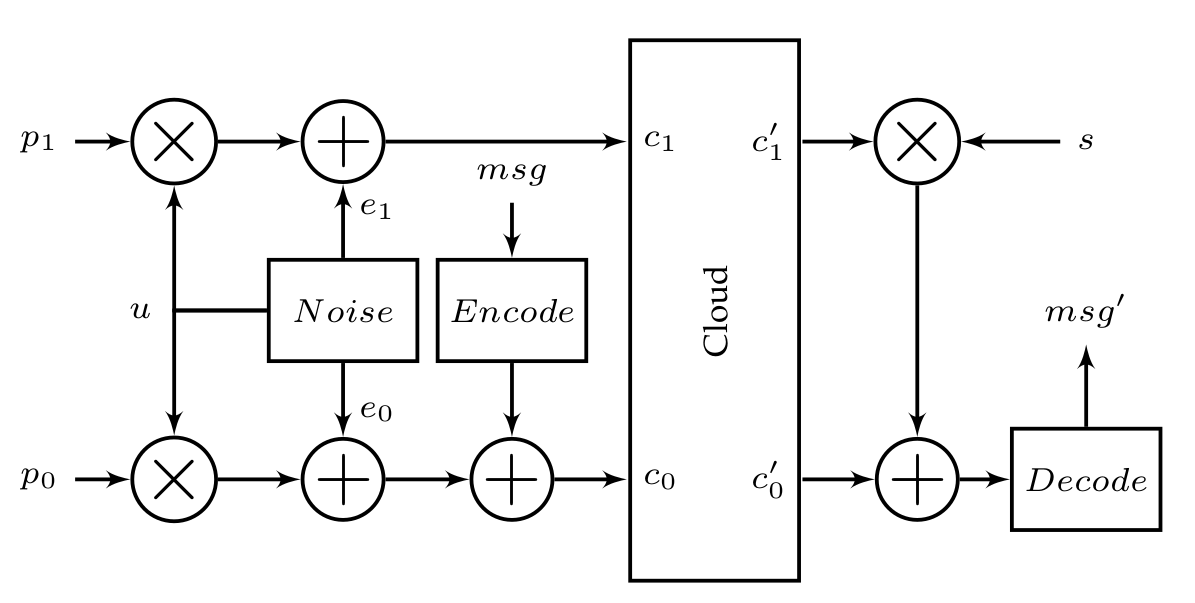
\includegraphics[scale=0.18]{fv.png}
%%  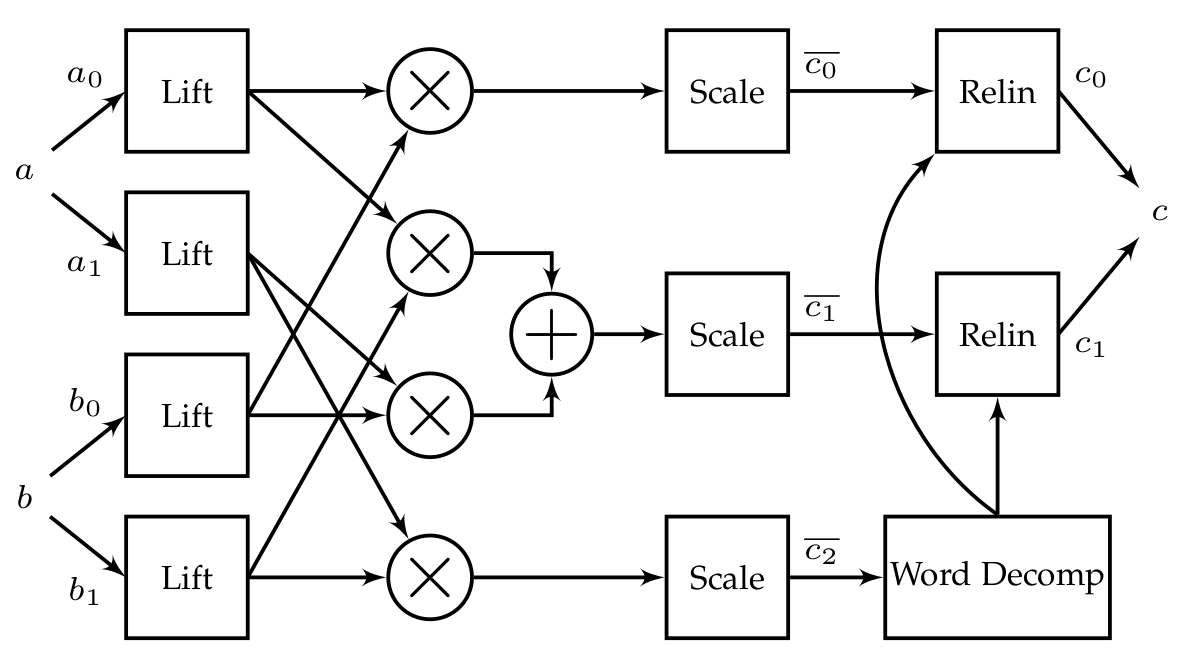
\includegraphics[scale=0.18]{fvhom.png}\\[-0.5em]
%%(a)\hspace{7.2cm}(b)
%%  \caption{(a) Fan and Vercauteren  (FV) encryption  encrypts a message into pair of ciphertexts c0 and c1 using public keys p0 and p1. 
%%  (b) Fan and Vercauteren homomorphic multiplication over the ciphertexts (figures are taken from \cite{turan2020heaws}.)}
%%  \label{hom}
%% \end{figure}
%% HE is based on lattice problems and adds noise during encryption. The value of this noise becomes greater each time an operation is performed on the ciphertext. 
%% Somewhat Homomorphic  Encryption (SHE) scheme only allows limited number of the operations on the ciphertext and more than that, the signal to noise ratio becomes so large that the original data could not be recovered anymore. Gentry in his paper introduced use of bootstrapping technique which is basically homomorphic evaluation of
%%the decryption circuit in the cloud to refresh and remove extra noises.
%% This resulted into Fully Homomorphic  Encryption (FHE). 
% However, such  operations are computationally expensive and increases the complexity of the homomorphic  computations circuit. 
%% Fig. \ref{hom} shows the circuit for homomorphic  encryption and homomorphic multiplication over encrypted data for  FV \citecrypto{fv} scheme. 
% Compared to software implementations, hardware cryptography results in a higher speed and a lower cost, while satisfying efficiency and low-power requirements of electronic
%devices. Implementation of homomorphic encryption and evaluation circuit is a extremely challenging because of the very large word length of ciphertexts and computational unit, specifically multipliers. Homomorphic encryption  is a rather new research topic and its hardware implementation is less explored. In the following, I discuss my approach towards this  problem to achieve a better hardware for practical homomorphic encryption and data processing. 
%%First, is studying the homomorphic encryption and computation to reduce their complexity and optimize them for hardware implementation. For instance, polynomial multiplication is 
%%one of  the operations that is frequently performed over very large size operands (eg. 4096 coefficients of 180-bit size  ) and plays a key role in overall performance and cost of the hardware. Therefore, it is  important to optimize these algorithm as much as possible before implementing on hardware. 
%%Second, is designing and efficient hardware architecture to encrypt and process data homomorphically. \\[0.2cm]
%\\{\bf Previous Research: }
%As postdoctoral fellow, I was working on the efficient  FPGA implementation of  finite field multipliers for Elliptic Curve Cryptography (ECC)  where we proposed a new binary polynomial multiplication algorithm with low complexity and high speed.
%The work was then extended to to hardware implementation of lattice based cryptography  algorithms and other post-quantum encryption algorithms.
%\\
%% Currently, I am closely monitoring PhD students researching in post quantum cryptography and homomorphic encryption where their research is focused on designing an FPGA based embedded processor for these algorithms.  \\
%{\bf Future Research (Research Plan): }
%My future research plan engages both studying and optimizing post quantum and homomorphic  encryption  and computation algorithms as well as designing an efficient embedded processor and processor for these algorithms. 
%%Towards this objectives, I defined 3 projects.\\[0.2cm]
%%{\bf Project 1}
%%
%%This project aims to study the different algorithms presented by researchers for 
%%post quantum cryptography including finalists of the NIST completion to standardize  quantum resistant public key cryptographic algorithms. The objective of this study is to reduce complexity and optimize these algorithms for FPGA implementation. 
%%\\[0.2cm]
%%{\bf Project 2}
%%
%%Investigating homomorphic encryption and ciphertext computation algorithms. Students will 
%%perform mathematical analysis to enhance these algorithm in the terms of area and delay complexity. Further, they will run computer simulations to check validity of the algorithms. 
%%\\[0.2cm]
%%{\bf Project 3}
%%
%%Students will design an architecture and circuit to efficiently implement  these algorithms on hardware, either as accelerator for computer software or possibly as an standalone hardware cryptography system.\\[0.2cm]
%\\{\bf Research Program Feasibility: }
%For the first phase which is optimizing  algorithms for hardware implementation, I will use Python programming language to run simulations and check the validity of  modified algorithms.  Further, I will use FPGAs as implementation platform to measure efficiency of design. FPGAs are substantially cheaper than designing  and fabricating a VLSI ASIC and have advantage of flexibility. Eventually, after testing design could be fabricated for final evaluations. Towards this objectives, I defined 3 projects:
% Project 1: 
%This project aims to study the different algorithms presented by researchers for 
%post quantum cryptography including finalists of the NIST completion to standardize  quantum resistant public key cryptographic algorithms. The objective of this study is to reduce complexity and optimize these algorithms for FPGA implementation. 
%{ Project 2:}
%Investigating homomorphic encryption and ciphertext computation algorithms. Students will 
%perform mathematical analysis to enhance these algorithm in the terms of area and delay complexity. Further, they will run computer simulations to check validity of the algorithms. 
%{ Project 3:}
%Students will design an architecture and circuit to efficiently implement  these algorithms on hardware, either as accelerator for computer software or possibly as an standalone hardware cryptography system.
%\\{\bf Funding for research }
%In terms of funding , I would be able to use my background and familiarity with problems and concerns of industry to secure funding for the research. I have also experience of writing successful research proposal with industry partner to obtain MITACS grant. \\ 
%\hspace*{-1.8em}
%{\bf References} \\
%%\vspace*{-4em}
%{\footnotesize
%\phantom \quad [1] J. Yoo and J. H. Yi, “Code-based authentication scheme for lightweight integrity checking of smart vehicles,” IEEE Access,
%vol. 6, pp. 46731–46741, 2018.\\[-0.1em]
%\phantom \quad [2] R. Abu-Salma, M. A. Sasse, J. Bonneau, A. Danilova, A. Naiakshina, and M. Smith, “Obstacles to the adoption of secure
%communication tools,” in 2017 IEEE Symposium on Security and Privacy (SP), pp. 137–153, 2017.\\[-0.1em]
%\phantom \quad [3] P. Aparna and P. V. V. Kishore, “Biometric-based efficient medical image watermarking in e-healthcare application,” IET
%Image Processing, vol. 13, no. 3, pp. 421–428, 2019.\\[-0.1em]
%\phantom \quad [4] T. D. P. Bai, K. M. Raj, and S. A. Rabara, “Elliptic curve cryptography based security framework for internet of things (iot)
%enabled smart card,” in 2017 World Congress on Computing and Communication Technologies (WCCCT), pp. 43–46, 2017.\\[-0.1em]
%\phantom \quad [5] P. W. Shor, "Algorithms for quantum computation: discrete logarithms and factoring," Proceedings 35th Annual Symposium on Foundations of Computer Science, 1994, pp. 124-134, doi: 10.1109/SFCS.1994.365700\\[-0.1em]
%\phantom \quad [6] “Post-Quantum Cryptography-Round 3 Submissions,” 2020.

%}
